\documentclass{article}
\usepackage[utf8]{inputenc}

\usepackage{amssymb}
\usepackage{enumitem}
\usepackage[hidelinks, pagebackref=true]{hyperref}
\usepackage{multicol}
\usepackage{authblk}
\usepackage{multirow}
\usepackage{mathtools}
\usepackage{float}
\usepackage{multicol}
\usepackage{graphicx}
\restylefloat{table}
\usepackage{caption}
\usepackage{subcaption}
\usepackage{caption, floatrow}
\usepackage{mathrsfs}
\usepackage{hyperref}
\usepackage{epstopdf}
\usepackage[margin=0.5in]{geometry}
\usepackage{amsmath}
\usepackage{floatrow}
\usepackage{caption}

\epstopdfDeclareGraphicsRule{.gif}{png}{.png}{convert gif:#1 png:\OutputFile}
\AppendGraphicsExtensions{.gif}

\newtheorem{definition}{Definition}
\newtheorem{lemma}{Lemma}
\newtheorem{sublemma}{Lemma}[lemma]






\title{\textbf{SimAN: Exploring Self-Supervised Representation Learning of Scene Text
via Similarity-Aware Normalization}}
\date{} % clear date
\author[1]{Canjie Luo}\author[1,2,*]{Lianwen Jin}\author[3]{Jingdong Chen}

\affil[1]{South China University of Technology,}
\affil[2]{Peng Cheng Laboratory,}
\affil[3]{Ant Group}







\begin{document}

\maketitle
 

\begin{multicols}{2}

    \begin{center}
        \textbf{Abstract}
    \end{center}
    Recently self-supervised representation learning has
    drawn considerable attention from the scene text recognition community. Different from previous studies using contrastive learning, we tackle the issue from an alternative
    perspective, i.e., by formulating the representation learning
    scheme in a generative manner. Typically, the neighboring image patches among one text line tend to have similar styles, including the strokes, textures, colors, etc. Motivated by this common sense, we augment one image patch
    and use its neighboring patch as guidance to recover itself.
    Specifically, we propose a Similarity-Aware Normalization
    (SimAN) module to identify the different patterns and align
    the corresponding styles from the guiding patch. In this
    way, the network gains representation capability for distinguishing complex patterns such as messy strokes and cluttered backgrounds. Experiments show that the proposed
    SimAN significantly improves the representation quality and
    achieves promising performance. Moreover, we surprisingly find that our self-supervised generative network has
    impressive potential for data synthesis, text image editing,
    and font interpolation, which suggests that the proposed
    SimAN has a wide range of practical applications.

    
    \section{Introduction}
        To summarize, our contributions are as follows:
        \begin{itemize}
            \item We propose a generative (opposite of contrastive [34])
            representation learning scheme by utilizing the unique
            properties of scene text, which might inspire rethinking the learning of better representations for sequential
            data like text images. To the best of our knowledge,
            this is the first attempt for scene text recognition.
            \item We propose a generative (opposite of contrastive [34])
            representation learning scheme by utilizing the unique
            properties of scene text, which might inspire rethinking the learning of better representations for sequential
            data like text images. To the best of our knowledge,
            this is the first attempt for scene text recognition mented image patch and its neighboring patch to align
            corresponding styles. Only if the representations are
            sufficiently distinguishable, different patterns can be
            identified and be aligned with correct styles. Otherwise, the network might result in a wrong recovered
            image, e.g., in different colors.
            \item The proposed SimAN achieves promising representation performance. Moreover, the self-supervised network shows impressive capabilities to synthesize data,
            edit text images and interpolate fonts, suggesting the
            broad practical applications of the proposed approach.
        \end{itemize}
    
    \setcounter{section}{2}
    
    
    
    \section{Methodology}
        In this section, we first introduce the design of the pretext
        task and the construction of the training samples. Then, we
        detail the proposed SimAN module. Finally, we present the
        objectives of the task and the complete learning scheme.
        The overall framework is shown in Figure \ref{fig:my_figure2}.
        \subsection{Training Sample Construction}
            Constructing appropriate training samples is critical to the success of the pretext task. We enable the scene text representation learning by recovering an augmented image patch using its neighboring patch as guidance. This design considers the unique properties of scene text, i.e., the styles (e.g., stroke width, textures, and colors) within one text line tend to be consistent.
    
            The pretext task requires decoupled style and content inputs. As shown in Figure \ref{fig:my_figure2}, given an unlabeled text image $I \in \mathbb{R}^{3 \times H \times W}$ (the width $W$ is required to be larger than two times of height $H$), we randomly crop two neighboring image patches $I_s, I_c \in \mathbb{R}^{3 \times H \times H}$ as style and content input, respectively. This ensures sufficient differences in content between the two patches. Even if the neighboring patches might contain a same characters, their positions are different. Then, we augment (blurring, random noise, color changes, etc.) the content patch $I_c$ as $I_{aug}$ to make its style different from the style patch $I_s$. Finally, the pretext task takes $I_{aug}$ as content input and $I_s$ as the style guidance to recover an image $I_{rec}$. The source content patch $I_c$ serves as supervision.
            \\
            
            \textbf{Discussion} As our pretext task is recovering an augmented patch under the guidance of its neighboring patch,
            the visual cues should be consistent in both patches. Some
            spatial augmentation strategies, such as elastic transformation, might break the consistency and lead to failed training.
            For instance, it might bring changes to the stroke width.
            The excessively distorted strokes are also diverse from the
            source font style. Therefore, we avoid all of the spatial
            transformation augmentation methods that are widely used
            for self-supervised representation learning. This is also a
            significant difference with previous study SeqCLR \cite{aberdam2021sequence}.
    
        \subsection{Similarity-Aware Normalization}
            Previous studies \cite{huang2017arbitrary,karras2019style} revealed that the statistics of
            feature maps, including mean and variance, can represent
            styles. Based on this finding, we perform instance normalization (IN) \cite{huang2017arbitrary,ulyanov2016instance} on the feature maps to remove the style
        \begin{equation}
        \tag{4}
          \sigma_{c,i,j}= \frac{1}{3} \sqrt{\sum_{p,q\in \mathbb{N}_{i,j}}(x_{c,p,q}-\mu_{c,i,j})^2},  
        \end{equation}
    
        \subsection{Learning Scheme}
            As we formulate the pretext task as image reconstruction, the source patch Ic can serves as supervision. We minimize the distance between the recovered image Irec and
            target image Ic as
            \begin{equation}
            \tag{8}
                 \mathcal{L}_{2}=\parallel I_{rec}-I{c} \parallel^2 _{2}.
            \end{equation}
            Simultaneously, we adopt a widely used adversarial objective to minimize the distribution shift between the generated and real data:
            \begin{equation}
            \tag{9}
                \min_{D} \mathcal{L}{adv} = \mathbb{E} \left[ \left(D(I_s) - 1 \right)^2 \right] + \mathbb{E} \left[ \left(D(I{rec}) \right)^2 \right]
            \end{equation}
            \begin{equation}
            \tag{10}
                \min_{\text{Encoder, Decoder}} \mathcal{L}_{adv} = \mathbb{E}\big[(D(I_{rec})-1)^2\big]
            \end{equation}
            where D denotes a discriminator.
            The complete learning scheme is shown in Algorithm 1.
            The encoder/decoder and discriminator are alternately optimized to achieve adversarial training
            \\
            \\
            \hline
            \textbf{Algorithm 1} Representation Learning Scheme
            \hline \\
            
            \textbf{Input:} Encoder, Decoder, Discriminator D
            
            \textbf{Output:}  Encoder, Decoder
            
            1: \textbf{for} iteration t = 0, 1, 2, ..., T \textbf{do}
            
            2: \hspace{0.5cm} Sample a mini-batch \{I_i\}_{i=1}^{B} 
            from unlabeled data 
            
            3: \hspace{0.5cm} for each I_i \textbf{do}
            
            4: \hspace{0.8cm} Randomly crop I_s and I_c, augment I_c as I_{aug}
            
            5: \hspace{0.5cm} Forward Encoder, SimAN and Decoder
            
            6: \hspace{0.5cm} Compute loss for \{I_{rec},i\}_{i=1}^{B}
            
            7: \hspace{0.5cm} Update D using \min_{D} \mathcal{L}{adv}
            
            8: Update Encoder and Decoder using \min_{\text{Encoder, Decoder}} \mathcal{L}_{adv}
            
            9: \hspace{0.5cm} (The \lambda is empirically set to 10.)
            
            \hline
    
    \setcounter{section}{3}
    
    \section{ Experiments}
        \subsection{Dataset}
        \subsection{Implementation Details}
            We provide more details, such as augmentations, architectures, probe objectives, and training settings, in the Supplementary Material.\newline
            \textbf{Encoder/Decoder} We adopt a popular recognizer backbone ResNet-29 [2] as our encoder. We symmetrically design a lightweight decoder.\newline
            \textbf{Recognizer} The complete architecture of the recognizer
            follows [1,2], including a rectification module, a ResNet-29
            backbone, two stacked BiLSTMs and a CTC [15] /Attention [4] decoder, as shown in Figure 3.\newline
            \textbf{Optimization} In the self-supervised representation
            learning stage, we set the batch size to 256 and train the
            network for 400K iterations. It takes less than 3 days for
            convergence on two NVIDIA P100 GPUs (16GB memory
            per GPU). The optimizer is Adam [30] with the settings
            of \beta_1 = 0.5 and \beta_2 = 0.999. The learning rate is set to
            10^{−4}
            and linearly decreased to 10^{−5}
            . The images are resized to a height of 32 pixels, maintaining the aspect ratio.
            The training setting of recognizers follows previous study
            SeqCLR [1].
    
            \newline
            \newline
            
    \textbf{Acknowledgment}\newline
        This research was supported in part by NSFC (Grant No.
        61936003) and GD-NSF (No. 2017A030312006).
    
     

\end{multicols}



\begin{table} [t]

    \captionsetup{justification=centering}
    \captionabove
    {
        Table 3. Probe evaluation. We report the word accuracy (Acc., \%)
        and word-level accuracy up to one edit distance (E.D. 1, \%). The
        real training data provides more robust representations.
    }
    \begin{center}
    \begin{tabular}{ c c c c c c c c c} 
     \hline
     Probe &  \multicolumn{2}{c}{Traning Data} &  \multicolumn{2}{c}{IIIT5K} &  \multicolumn{2}{c}{IC03} & \multicolumn{2}{c}{IC13} \\ 
     \cline{2-3}   \cline{4-5}  \cline{6-7} \cline{8-9}
    Type & Encoder & Probe & Acc. & E.D.1 & Acc. & E.D.1 & Acc. & E.D.1\\ 
    \hline
    \multirow{2}{*}{CTC} & Synth. & Synth. & 60.8 & 75.6 & 64.9 & 78.9 & 64.0 & 81.0\\
    & Real. & Synth. & \textbf{68.9} & \textbf{82.8} & \textbf{75.0} & \textbf{87.2} & \textbf{72.9} & \textbf{86.0}\\
    \hline
    \multirow{2}{*}{Att.} & Synth. & Synth. & 66.5 & 78.8 & 71.7 & 83.6 & 68.7 & 81.6\\
    & Real. & Synth. & \textbf{73.7} & \textbf{85.6} & \textbf{81.2} & \textbf{90.4} & \textbf{77.9} & \textbf{87.8}\\
    \hline
    \end{tabular}
    \end{center}
     
    \label{tab:my_label2}
    
\end{table}

\begin{table} [t]

    \captionsetup{justification=centering}
    \captionabove
    {
        Table 6. Arbitrary-length Text editing evaluation. We report FID
        score and word-level recognition accuracy (\%). Although the supervised EditText can imitate more font category and background
        texture, our self-supervised approach achieves better readability.
    }
    \begin{center}
    \begin{tabular}{ c c c c } 
     \hline
        Method & Supervision & FID$\downarrow$ & Acc.$\uparrow$ \\ 
        EditText[57] & $\checkmark$ & \textbf{40.5} & 14.9\\ 
        Ours & $\times$ & 67.9 & \textbf{57.6} \\ 
     \hline
    \end{tabular}
    \end{center}
     
    \label{tab:my_label1}
    
\end{table}






\begin{figure}
    \centering
    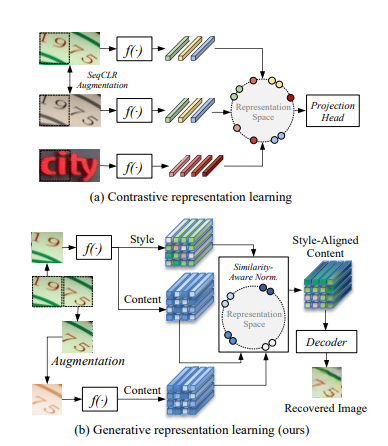
\includegraphics[width=0.5\textwidth]{f1.PNG}
    \caption
    { 
        Scene text representation learning in (a) the contrastive
        and (b) the generative manner (ours). We estimate the similarity
        of the content representations between the augmented patch and
        its neighboring patch, and align the corresponding styles to reconstruct the augmented patch. Only high-quality representations are
        distinguishable so that a precise reconstruction can be achieved
    }
    \label{fig:my_figure1}
\end{figure}


\begin{figure}
    \centering
    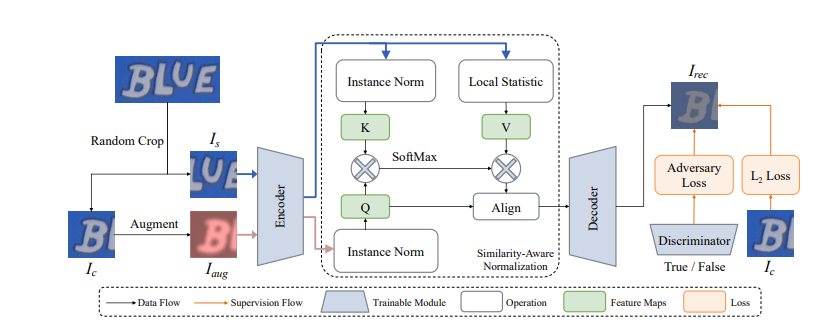
\includegraphics[width=0.5\textwidth]{f2.PNG}
    \caption
    {
        Overview of the proposed generative representation learning scheme. We decouple content and style as two different inputs and
        guide the network to recover the augmented image. The proposed SimAN module learns to align corresponding styles for different patterns
        according to the distinguishable representations.
    }
    
    \label{fig:my_figure2}
\end{figure}

\setcounter{figure}{4}

\begin{figure}
    \centering
    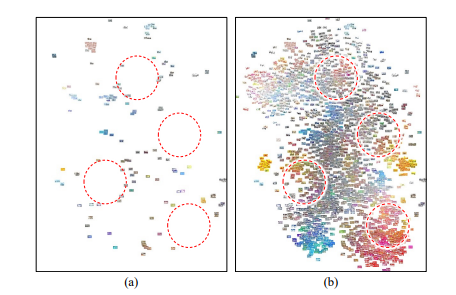
\includegraphics[width=0.5\textwidth]{f5.PNG}
    \caption
    { 
        Distribution of scene text images containing the word
        “the” via t-SNE. We show two distributions of (a) 200 real labeled
        samples and (b) 200 real samples and our 2000 synthetic samples.
        The large empty space of original distribution might suggest the
        lack of diversity of labeled data. After adding our synthetic samples, the distribution is more even and dense. Best viewed in color
    }
    \label{fig:my_figure5}
\end{figure}

\bibliographystyle{plain}
\bibliography{resource.bib}

\end{document}
